%%%%%%%%%%%%%%%%%%%%%%%%%%%%%%%%%%%%%%%%%%%%%%%%%%%%%%%%%%%%%%%
%% OXFORD THESIS TEMPLATE

% Use this template to produce a standard thesis that meets the Oxford University requirements for DPhil submission
%
% Originally by Keith A. Gillow (gillow@maths.ox.ac.uk), 1997
% Modified by Sam Evans (sam@samuelevansresearch.org), 2007
% Modified by John McManigle (john@oxfordechoes.com), 2015
% Modified by Ulrik Lyngs (ulrik.lyngs@cs.ox.ac.uk), 2018-, for use with R Markdown
%
% Ulrik Lyngs, 25 Nov 2018: Following John McManigle, broad permissions are granted to use, modify, and distribute this software
% as specified in the MIT License included in this distribution's LICENSE file.
%
% John commented this file extensively, so read through to see how to use the various options.  Remember that in LaTeX,
% any line starting with a % is NOT executed.  Several places below, you have a choice of which line to use
% out of multiple options (eg draft vs final, for PDF vs for binding, etc.)  When you pick one, add a % to the beginning of
% the lines you don't want.


%%%%% PAGE LAYOUT
% The most common choices should be below.  You can also do other things, like replacing "a4paper" with "letterpaper", etc.

% This one formats for two-sided binding (ie left and right pages have mirror margins; blank pages inserted where needed):
%\documentclass[a4paper,twoside]{templates/ociamthesis}
% This one formats for one-sided binding (ie left margin > right margin; no extra blank pages):
%\documentclass[a4paper]{ociamthesis}
% This one formats for PDF output (ie equal margins, no extra blank pages):
%\documentclass[a4paper,nobind]{templates/ociamthesis}

% As you can see from the uncommented line below, oxforddown template uses the a4paper size, 
% and passes in the binding option from the YAML header in index.Rmd:
\documentclass[a4paper, $if(page-layout)$$page-layout$$endif$]{templates/ociamthesis}


%%%%% ADDING LATEX PACKAGES
% add hyperref package with options from YAML %
\usepackage[pdfpagelabels]{hyperref}
% change the default coloring of links to something sensible
\usepackage{xcolor}

$if(linkcolor-rgb)$
\definecolor{mylinkcolor}{RGB}{$linkcolor-rgb$}
$endif$
$if(urlcolor-rgb)$
\definecolor{myurlcolor}{RGB}{$urlcolor-rgb$}
$endif$
$if(citecolor-rgb)$
\definecolor{mycitecolor}{RGB}{$citecolor-rgb$}
$endif$

$if(colored-not-bordered-links)$
\hypersetup{
  hidelinks,
  colorlinks,
  linktocpage=$if(toc-link-page-numbers)$$toc-link-page-numbers$$else$false$endif$,
  linkcolor=$if(linkcolor-rgb)$mylinkcolor$else$.$endif$,
  urlcolor=$if(urlcolor-rgb)$myurlcolor$else$.$endif$,
  citecolor=$if(citecolor-rgb)$mycitecolor$else$.$endif$
}

$else$
\hypersetup{
  colorlinks=false,
  linktocpage=$if(link-toc-page)$$link-toc-page$$else$true$endif$,
  linkbordercolor=$if(linkcolor-rgb)$mylinkcolor$else$.$endif$,
  urlbordercolor=$if(urlcolor-rgb)$myurlcolor$else$.$endif$,
  citebordercolor=$if(citecolor-rgb)$mycitecolor$else$.$endif$
}
$endif$


% add float package to allow manual control of figure positioning %
\usepackage{float}

% enable strikethrough
\usepackage[normalem]{ulem}

% use soul package for correction highlighting
\usepackage{color, soulutf8}
\definecolor{correctioncolor}{HTML}{CCCCFF}
\sethlcolor{correctioncolor}
\newcommand{\ctext}[3][RGB]{%
  \begingroup
  \definecolor{hlcolor}{#1}{#2}\sethlcolor{hlcolor}%
  \hl{#3}%
  \endgroup
}
\soulregister\ref7
\soulregister\cite7
\soulregister\citet7
\soulregister\autocite7
\soulregister\textcite7
\soulregister\pageref7

% enable wrapping of URLs stretching over two lines
\usepackage{xurl}

% enable UTF8 
\usepackage[utf8]{inputenc}

% enable adding PDFs
\usepackage{pdfpages}

%%%%% FIXING / ADDING THINGS THAT'S SPECIAL TO R MARKDOWN'S USE OF LATEX TEMPLATES
% pandoc puts lists in 'tightlist' command when no space between bullet points in Rmd file,
% so we add this command to the template
\providecommand{\tightlist}{%
  \setlength{\itemsep}{0pt}\setlength{\parskip}{0pt}}
 
% UL 1 Dec 2018, fix to include code in shaded environments
$if(highlighting-macros)$
$highlighting-macros$

%UL set white space before and after code blocks
\renewenvironment{Shaded}
{
  \vspace{$space-before-code-block$}%
  \begin{snugshade}%
}{%
  \end{snugshade}%
  \vspace{$space-after-code-block$}%
}
$endif$

% User-included things with header_includes or in_header will appear here
% kableExtra packages will appear here if you use library(kableExtra)
$for(header-includes)$
$header-includes$
$endfor$


%UL set section header spacing
\usepackage{titlesec}
% 
\titlespacing\subsubsection{0pt}{24pt plus 4pt minus 2pt}{0pt plus 2pt minus 2pt}


%UL set whitespace around verbatim environments
\usepackage{etoolbox}
\makeatletter
\preto{\@verbatim}{\topsep=0pt \partopsep=0pt }
\makeatother


%%%%%%% PAGE HEADERS AND FOOTERS %%%%%%%%%
\usepackage{fancyhdr}
\setlength{\headheight}{15pt}
\fancyhf{} % clear the header and footers
\pagestyle{fancy}
\renewcommand{\chaptermark}[1]{\markboth{\thechapter. #1}{\thechapter. #1}}
\renewcommand{\sectionmark}[1]{\markright{\thesection. #1}} 
\renewcommand{\headrulewidth}{0pt}

$if(running-header)$
\fancy$running-header-foot-or-head$[$running-header-position-leftmark$]{\emph{\leftmark}} 
\fancy$running-header-foot-or-head$[$running-header-position-rightmark$]{\emph{\rightmark}} 
$endif$

% UL page number position 
\fancy$ordinary-page-number-foot-or-head$[$ordinary-page-number-position$]{\emph{\thepage}} %regular pages
\fancypagestyle{plain}{\fancyhf{}\fancy$chapter-page-number-foot-or-head$[$chapter-page-number-position$]{\emph{\thepage}}} %chapter pages

% JEM fix header on cleared pages for openright
\def\cleardoublepage{\clearpage\if@twoside \ifodd\c@page\else
   \hbox{}
   \fancy$ordinary-page-number-foot-or-head$[$ordinary-page-number-position$]{}
   \newpage
   \if@twocolumn\hbox{}\newpage
   \fi
   \fancy$running-header-foot-or-head$[$running-header-position-leftmark$]{\emph{\leftmark}} 
   \fancy$running-header-foot-or-head$[$running-header-position-rightmark$]{\emph{\rightmark}} 
   \fi\fi}


%%%%% SELECT YOUR DRAFT OPTIONS
% This adds a "DRAFT" footer to every normal page.  (The first page of each chapter is not a "normal" page.)
$if(draft-mark)$
\fancy$draft-mark-foot-or-head$[$draft-mark-position$]{\emph{DRAFT Printed on \today}}
$endif$

% IP feb 2021: option to include line numbers in PDF
$if(includeline-num)$
\usepackage{lineno}
\linenumbers
$endif$

% for line wrapping in code blocks
$if(line-wrapping-in-code)$
\usepackage{fvextra}
\DefineVerbatimEnvironment{Highlighting}{Verbatim}{breaklines,commandchars=\\\{\}}
$endif$

% This highlights (in blue) corrections marked with (for words) \mccorrect{blah} or (for whole
% paragraphs) \begin{mccorrection} . . . \end{mccorrection}.  This can be useful for sending a PDF of
% your corrected thesis to your examiners for review.  Turn it off, and the blue disappears.
$if(corrections)$
\correctionstrue
$endif$


%%%%% BIBLIOGRAPHY SETUP
% Note that your bibliography will require some tweaking depending on your department, preferred format, etc.
% If you've not used LaTeX before, I recommend reading a little about biblatex/biber and getting started with it.
% If you're already a LaTeX pro and are used to natbib or something, modify as necessary.
% Either way, you'll have to choose and configure an appropriate bibliography format...

% this enables pandoc citations
$if(csl-refs)$
\newlength{\cslhangindent}
\setlength{\cslhangindent}{1.5em}
\newlength{\csllabelwidth}
\setlength{\csllabelwidth}{3em}
\newlength{\cslentryspacingunit} % times entry-spacing
\setlength{\cslentryspacingunit}{\parskip}
\newenvironment{CSLReferences}[2] % #1 hanging-ident, #2 entry spacing
 {% don't indent paragraphs
  \setlength{\parindent}{0pt}
  % turn on hanging indent if param 1 is 1
  \ifodd #1
  \let\oldpar\par
  \def\par{\hangindent=\cslhangindent\oldpar}
  \fi
  % set entry spacing
  \setlength{\parskip}{$refs-space-between-entries$}
  \setlength{\baselineskip}{$refs-line-spacing$}
 }%
 {}
\usepackage{calc}
\newcommand{\CSLBlock}[1]{#1\hfill\break}
\newcommand{\CSLLeftMargin}[1]{\parbox[t]{\csllabelwidth}{#1}}
\newcommand{\CSLRightInline}[1]{\parbox[t]{\linewidth - \csllabelwidth}{#1}\break}
\newcommand{\CSLIndent}[1]{\hspace{\cslhangindent}#1}
$endif$

$if(use-biblatex)$
\usepackage[$bib-latex-options$]{biblatex}

$for(bibliography)$
\addbibresource{$bibliography$}
$endfor$

% This makes the bibliography left-aligned (not 'justified') and slightly smaller font.
\renewcommand*{\bibfont}{\raggedright\small}

$endif$

$if(use-natbib)$
\usepackage{natbib}
\setcitestyle{$natbib-citation-style$}
\bibliographystyle{$natbib-bibliography-style$}
\addto\captionsenglish{%
  \renewcommand{\bibname}{}
  \renewcommand{\bibsection}{}
}

% This makes the bibliography left-aligned (not 'justified') and slightly smaller font.
\renewcommand*{\bibfont}{\raggedright\small}

$endif$


% Uncomment this if you want equation numbers per section (2.3.12), instead of per chapter (2.18):
%\numberwithin{equation}{subsection}


%%%%% THESIS / TITLE PAGE INFORMATION
% Everybody needs to complete the following:
\title{$title$}
\author{$author$}
\college{$college$}

% Master's candidates who require the alternate title page (with candidate number and word count)
% must also un-comment and complete the following three lines:
$if(masters-submission)$
\masterssubmissiontrue
\candidateno{$candidate-number$}
\wordcount{$word-count$}
$endif$

% Uncomment the following line if your degree also includes exams (eg most masters):
%\renewcommand{\submittedtext}{Submitted in partial completion of the}
% Your full degree name.  (But remember that DPhils aren't "in" anything.  They're just DPhils.)
\degree{$degree$}
% Term and year of submission, or date if your board requires (eg most masters)
\degreedate{$degreedate$}


%%%%% YOUR OWN PERSONAL MACROS
% This is a good place to dump your own LaTeX macros as they come up.

% To make text superscripts shortcuts
	\renewcommand{\th}{\textsuperscript{th}} % ex: I won 4\th place
	\newcommand{\nd}{\textsuperscript{nd}}
	\renewcommand{\st}{\textsuperscript{st}}
	\newcommand{\rd}{\textsuperscript{rd}}

%%%%% THE ACTUAL DOCUMENT STARTS HERE
\begin{document}

%%%%% CHOOSE YOUR LINE SPACING HERE
% This is the official option.  Use it for your submission copy and library copy:
\setlength{\textbaselineskip}{$linespacing$}
% This is closer spacing (about 1.5-spaced) that you might prefer for your personal copies:
%\setlength{\textbaselineskip}{18pt plus2pt minus1pt}

% You can set the spacing here for the roman-numbered pages (acknowledgements, table of contents, etc.)
\setlength{\frontmatterbaselineskip}{$frontmatter-linespacing$}

% UL: You can set the line and paragraph spacing here for the separate abstract page to be handed in to Examination schools
\setlength{\abstractseparatelineskip}{13pt plus1pt minus1pt}
\setlength{\abstractseparateparskip}{0pt plus 1pt}

% UL: You can set the general paragraph spacing here - I've set it to 2pt (was 0) so
% it's less claustrophobic
\setlength{\parskip}{2pt plus 1pt}

%
% Customise title page
%
$if(university-logo)$
\def\crest{{\includegraphics[width=$university-logo-width$]{$university-logo$}}}
$else$
\def\crest{}
$endif$
\renewcommand{\university}{$university$}
\renewcommand{\submittedtext}{$submitted-text$}
\renewcommand{\thesistitlesize}{\fontsize{$title-size$}{$title-size-linespacing$}\selectfont}
\renewcommand{\gapbeforecrest}{$gap-before-crest$}
\renewcommand{\gapaftercrest}{$gap-after-crest$}


% Leave this line alone; it gets things started for the real document.
\setlength{\baselineskip}{\textbaselineskip}


%%%%% CHOOSE YOUR SECTION NUMBERING DEPTH HERE
% You have two choices.  First, how far down are sections numbered?  (Below that, they're named but
% don't get numbers.)  Second, what level of section appears in the table of contents?  These don't have
% to match: you can have numbered sections that don't show up in the ToC, or unnumbered sections that
% do.  Throughout, 0 = chapter; 1 = section; 2 = subsection; 3 = subsubsection, 4 = paragraph...

% The level that gets a number:
\setcounter{secnumdepth}{$section-numbering-depth$}
% The level that shows up in the ToC:
\setcounter{tocdepth}{$toc-depth$}
% The level that shows up in the miniToCs"
\setcounter{minitocdepth}{1}


%%%%% ETHICS CERTIFICATE

\includepdf[pages=-]{inserted-PDFs/ethics-certificate.pdf}

%%%%% CANDIDATE'S DECLARATION
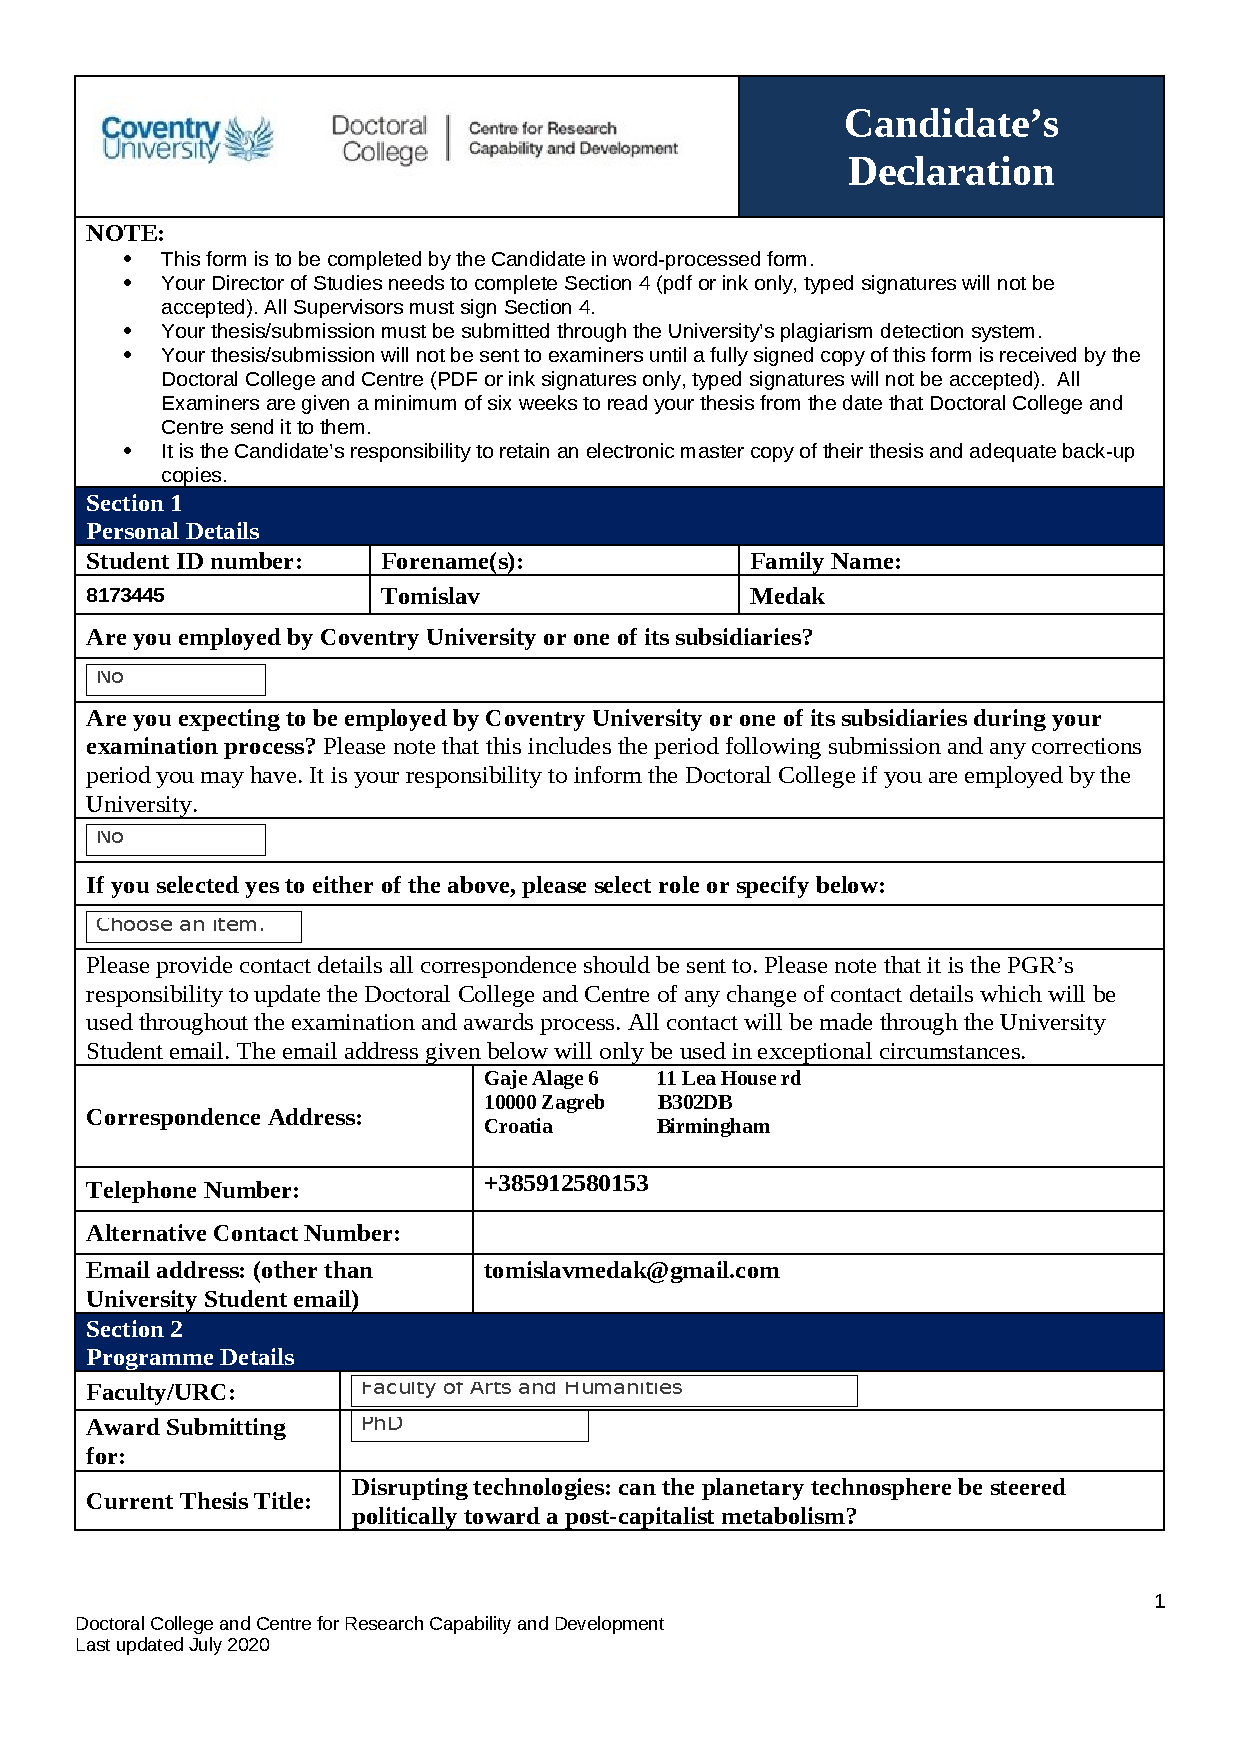
\includepdf[pages=-]{inserted-PDFs/candidates-declaration.pdf}


%%%%% ABSTRACT SEPARATE
% This is used to create the separate, one-page abstract that you are required to hand into the Exam
% Schools.  You can comment it out to generate a PDF for printing or whatnot.
$if(abstractseparate)$
\begin{abstractseparate}
  $abstract$
\end{abstractseparate}
$endif$

% JEM: Pages are roman numbered from here, though page numbers are invisible until ToC.  This is in
% keeping with most typesetting conventions.
\begin{romanpages}

% Title page is created here
$if(alternative-title-page)$
\input{$alternative-title-page$}
$else$
\maketitle
$endif$

%%%%% ABSTRACT
$if(abstract)$

$if(show-abstract-in-toc)$
\addcontentsline{toc}{chapter}{$abstract-heading$}
\renewcommand{\numberstyleabstract}{plain}
$endif$

\renewcommand{\abstracttitle}{$abstract-heading$}
\begin{abstract}
	$abstract$
\end{abstract}

$endif$

$if(abstract-second)$

$if(show-abstract-in-toc)$
\addcontentsline{toc}{chapter}{$abstract-second-heading$}
\renewcommand{\numberstyleabstract}{plain}
$endif$

\renewcommand{\abstractsecondtitle}{$abstract-second-heading$}
\begin{abstractsecond}
	$abstract-second$
\end{abstractsecond}

$endif$

%%%%% DEDICATION
$if(dedication)$
\begin{dedication}
  $dedication$
\end{dedication}
$endif$

%%%%% ACKNOWLEDGEMENTS
$if(acknowledgements)$

$if(show-acknowledgements-in-toc)$
\addcontentsline{toc}{chapter}{Acknowledgements}
\renewcommand{\numberstyleacks}{plain}
\renewcommand{\numberstyleabstract}{plain}
$endif$

\begin{acknowledgements}
 	$acknowledgements$
\end{acknowledgements}

$endif$


%%%%% MINI TABLES
% This lays the groundwork for per-chapter, mini tables of contents.  Comment the following line
% (and remove \minitoc from the chapter files) if you don't want this.  Un-comment either of the
% next two lines if you want a per-chapter list of figures or tables.
$if(mini-toc)$
  \dominitoc % include a mini table of contents
$endif$
$if(mini-lof)$
  \dominilof  % include a mini list of figures
$endif$
$if(mini-lot)$
  \dominilot  % include a mini list of tables
$endif$

% This aligns the bottom of the text of each page.  It generally makes things look better.
\flushbottom

% This is where the whole-document ToC appears:
\tableofcontents

$if(lof)$
\listoffigures
	\mtcaddchapter
  	% \mtcaddchapter is needed when adding a non-chapter (but chapter-like) entity to avoid confusing minitoc
$endif$

% Uncomment to generate a list of tables:
$if(lot)$
\listoftables
  \mtcaddchapter
$endif$

%%%%% LIST OF ABBREVIATIONS
% This example includes a list of abbreviations.  Look at text/abbreviations.tex to see how that file is
% formatted.  The template can handle any kind of list though, so this might be a good place for a
% glossary, etc.
$if(abbreviations)$
% First parameter can be changed eg to "Glossary" or something.
% Second parameter is the max length of bold terms.
\begin{mclistof}{$abbreviations-heading$}{$abbreviations-width$}

$abbreviations$

\end{mclistof} 

$endif$

% The Roman pages, like the Roman Empire, must come to its inevitable close.
\end{romanpages}

%%%%% CHAPTERS
% Add or remove any chapters you'd like here, by file name (excluding '.tex'):
\flushbottom

% all your chapters and appendices will appear here
$body$

%%%%% REFERENCES
$if(use-biblatex)$
\setlength{\baselineskip}{0pt} % JEM: Single-space References

% we are setting the title for the references section in front-and-back-matter/99-references_heading.Rmd
{\renewcommand*\MakeUppercase[1]{#1}%
\printbibliography[heading="References"]}

$endif$

$if(use-natbib)$
\bibliography{$for(bibliography)$$bibliography$$sep$,$endfor$}
$endif$

% set the section header to the references heading
\markboth{$params.referenceHeading$}{}

\end{document}
